\chapter{Stand der Technik}\label{chap:stand_der_technik}

\section{Grundlagen}

\subsection{Modell}
\label{subsec:modell}

Ein Modell ist das Ergebnis eines Trainingsprozesses, bei dem aus einer großen Menge von Beispieldaten Muster und Zusammenhänge gelernt werden und dabei die Modellparameter angepasst werden. 
Das dabei erlernte Wissen wird im Modell gespeichert und kann anschließend genutzt werden, um neue Eingaben zu verarbeiten und passende Vorhersagen zu erzeugen. 
Ein Modell bildet somit die Grundlage dafür, bereits gelernte Zusammenhänge auf bisher unbekannte Daten anzuwenden \parencite{LeCun2015}.

\subsection{Neuronale Netze}

Ein Neuronales Netz wie in Abbildung \ref{fig:neuronales_netz} dargestellt, ist ein Netzwerk aus miteinander verbundenen Knoten, den sogenannten Neuronen, die in ihrer Struktur und Funktionsweise an das menschliche Gehirn angelehnt sind.
Diese Neuronen sind durch Verbindungen miteinander Verknüpft, die die Stärke der Signalübertragung zwischen den Neuronen bestimmen. 
Ein Neuronales Netz besteht aus mehreren Schichten von Neuronen wie Eingabeschicht, versteckten Schichten und Ausgabeschicht.
Diese Schichten arbeiten zusammen und verarbeiten die Eingaben wie Text, Bilder oder Sensordaten schrittweise.
Jede Schicht hat dabei eine spezifische Funktion: Die Eingabeschicht nimmt die Rohdaten auf, die versteckten Schichten extrahieren Merkmale und Muster, und die Ausgabeschicht liefert die endgültigen Vorhersagen für den jeweiligen Anwendungsfall.
Während dem Lernens, dem sogenannten Training werden die Verbindungen und deren Gewichtungen zwischen den Neuronen schrittweise angepasst, 
sodass das Modell in der Lage ist, Muster und Zusammenhänge in den Eingaben zu erkennen \parencite{LeCun2015}.

\begin{figure}[ht] 
  \centering 
  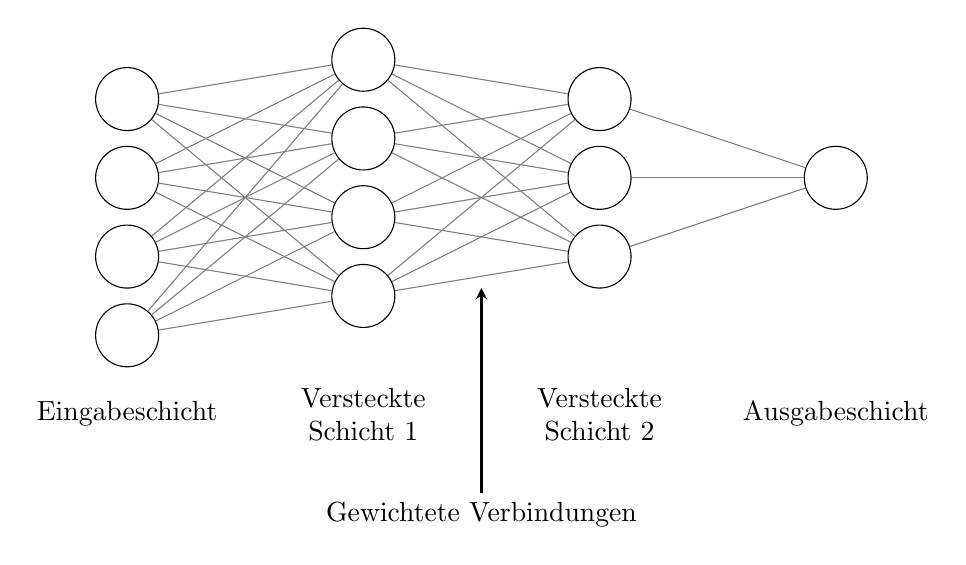
\begin{tikzpicture}[ neuron/.style={ circle, draw, minimum size=0.8cm }, >=stealth ] 
    % Eingabeschicht 
    \node[neuron] (i1) at (0,2) {}; 
    \node[neuron] (i2) at (0,1) {}; 
    \node[neuron] (i3) at (0,0) {}; 
    \node[neuron] (i4) at (0,-1) {}; 
    % Hidden Layer 1 
    \node[neuron] (h11) at (3,2.5) {}; 
    \node[neuron] (h12) at (3,1.5) {}; 
    \node[neuron] (h13) at (3,0.5) {}; 
    \node[neuron] (h14) at (3,-0.5) {}; 
    % Hidden Layer 2 
    \node[neuron] (h21) at (6,2) {}; 
    \node[neuron] (h22) at (6,1) {}; 
    \node[neuron] (h23) at (6,0) {}; 
    % Ausgabeschicht 
    \node[neuron] (o1) at (9,1) {}; 
    % Verbindungen Input -> Hidden 1 
    \foreach \i in {1,2,3,4} { 
      \foreach \h in {1,2,3,4} { 
        \draw[gray] (i\i) -- (h1\h); 
      } 
    } 
    % Verbindungen Hidden 1 -> Hidden 2 
    \foreach \h in {1,2,3,4} { 
      \foreach \k in {1,2,3} { 
        \draw[gray] (h1\h) -- (h2\k); 
      } 
    } 
    % Verbindungen Hidden 2 -> Output 
    \foreach \k in {1,2,3} { 
      \draw[gray] (h2\k) -- (o1); 
    } 
    % Beschriftungen 
    \node[align=center] at (0,-2) {Eingabeschicht}; 
    \node[align=center] at (3,-2) {Versteckte\\Schicht 1}; 
    \node[align=center] at (6,-2) {Versteckte\\Schicht 2}; 
    \node[align=center] at (9,-2) {Ausgabeschicht}; 
    % Pfeil für gewichtete Verbindungen 
    \draw[->, thick] (4.5,-3) -- (4.5,-0.4);
    \node[below] at (4.5,-3) {Gewichtete Verbindungen}; 
  \end{tikzpicture} 
  \caption{Schematischer Aufbau eines mehrschichtigen neuronalen Netzes} 
  \label{fig:neuronales_netz} 
\end{figure}


\subsection{Vektoren, Vektorraum, Embeddings und Embedding-Raum}

Vektoren sind geordnete Mengen von Zahlen, die in der Mathematik und Informatik verwendet werden, um Objekte im mehrdimensionalen Vektorraum darzustellen. 
In der Verarbeitung natürlicher Sprache werden Wörter, Sätze und Dokumente häufig in Vektoren überführt.
Ein anderes Wort für diese Vektoren ist Embeddings. Embeddings ermöglichen es, semantische Ähnlichkeiten zwischen Wörtern zu erfassen, indem ähnliche Wörter im mehrdimensionalen Embedding-Raum (vergleiche Abbildung \ref{fig:embedding3d}) nahe beieinander liegen.
Der Embedding-Raum ist der mehrdimensionale Raum, in dem diese Embeddings angeordnet sind. 
In diesem Raum repräsentieren die Positionen der Embeddings die semantischen Beziehungen zwischen den entsprechenden Wörtern. 
Jedes Wort wird dabei durch mehrere Zahlenwerte, die verschiedene Merkmale des Wortes repräsentieren, in einem Embedding dargestellt.
Die einzelnen Dimensionen eines Embeddings besitzen hier keine direkte, für Menschen verständliche Bedeutung.
Erst die Position der Embeddings im Raum ermöglicht es, semantische Ähnlichkeiten zwischen Wörtern zu erkennen \parencite{Mikolov2013}.

Ein Embedding kann dabei wie folgt veranschaulicht werden:

\[ \mathbf{e}_{\text{Katze}} = \begin{bmatrix} 0.82 \\ -0.15 \\ 0.47 \end{bmatrix} \]

Dieses Embedding repräsentiert das Wort „Katze“ im mehrdimensionalen Embedding-Raum, wobei jede Komponente des Vektors ein bestimmtes Merkmal oder eine Eigenschaft des Wortes „Katze“ kodiert.
Um die Funktionalität von Embeddings weiter zu verdeutlichen, sollen hier mehrere Embeddings für verschiedene Wörter exemplarisch betrachtet werden:

\[ 
\mathbf{e}_{\text{Katze}} 
= 
\begin{bmatrix} 
  0.82\\ 
  -0.15\\ 
  0.47 
\end{bmatrix}, 
\qquad 
\mathbf{e}_{\text{Hund}} 
= 
\begin{bmatrix} 
  0.79\\ 
  -0.12\\ 
  0.51 
\end{bmatrix}, 
\qquad 
\mathbf{e}_{\text{Auto}} 
= 
\begin{bmatrix} 
  -0.34\\ 
  0.88\\ 
  0.70 
\end{bmatrix} 
\]

Abbildung \ref{fig:embedding3d} zeigt die Position dieser Embeddings in einem vereinfachten dreidimensionalen Embedding-Raum. 
Da die Koordinaten der Wörter „Katze“ und „Hund“ sehr ähnlich sind, liegen ihre Positionen nahe beieinander. 
Das Embedding des Wortes „Auto“ unterscheidet sich dagegen stärker von „Katze“ oder „Hund“ und befindet sich deshalb weiter entfernt. 

\begin{figure}[ht] 
  \centering 
  \tdplotsetmaincoords{70}{115} 
  \begin{tikzpicture}[tdplot_main_coords, scale=3] 
    % Achsen 
    \draw[->] (-0.6,0,0) -- (1.1,0,0) node[right] {x}; 
    \draw[->] (0,-0.4,0) -- (0,1.1,0) node[left] {y}; 
    \draw[->] (0,0,-0.4) -- (0,0,0.8) node[above] {z}; 
    % Katze 
    \filldraw[blue] (0.82,-0.15,0.47) circle (1pt) node[above left] {Katze}; 
    % Hund 
    \filldraw[blue] (0.79,-0.12,0.51) circle (1pt) node[right] {Hund}; 
    % Auto 
    \filldraw[red] (-0.34,0.88,0.70) circle (1pt) node[left] {Auto}; 
  \end{tikzpicture} 
  \caption{Vereinfachte Darstellung der Beispiel-Embeddings im dreidimensionalen Embedding-Raum} 
  \label{fig:embedding3d} 
\end{figure}


\section {Modellansätze}

\subsection{Neural Language Models}

Neuronale Sprachmodelle (Neural Language Models, NLMs) sind spezielle neuronale Netze, die auf Textsammlungen, 
sogenannten Textkorpora, vortrainiert werden, um sprachliche Muster, semantische Zusammenhänge sowie Wissensrepräsentationen zu erlernen.
Hierzu werden Wörter, Sätze und Dokumente in Embeddings überführt, die als Eingabe für das neuronale Netz dienen \parencite{LeCun2015}.

\subsection{Large Language Models }

Large Language Models (LLMs) basieren auf neuronalen Sprachmodellen und erweitern diese durch eine enorme Anzahl an Parametern sowie tieferen Architekturen.
Sie bilden die Grundlage für generative KI-Systeme und ermöglichen die Bearbeitung von verschiedenen Aufgaben aus dem bereich der natürlichen Sprachverarbeitung.
Dazu zählen Textgenerierung, Textklassifikation, Frage-Antwort-Systeme sowie das liefern mehrer relevanter Ergebnisse zu einer Suchanfrage, dem sogenannten Information Retrieval \parencite{Zhao2023}.

Moderne LLMs bestehen typischerweise aus mehreren Milliarden Parametern. Während des Trainings werden hierbei diese Modellparameter wie in \autoref{subsec:modell} beschrieben auf Zusammenhänge gelernt. 
Diese Zusammenhänge beziehen sich hier auf die statistischen Beziehungen zwischen Wörtern, Sätzen und Dokumenten.
Dadurch können LLMs Aufgaben Lösen, auf die sie nicht explizit trainiert wurden, da die Antwort auf eine Eingabe aus dem erlernten Wissen abgeleitet werden kann. 
Hierbei spielt die Generalisierungsfähigkeit des Modells eine entscheidende Rolle. Anhand dieser Fähigkeit wird die Leistungsfähigkeit eines LLMs bei der Bearbeitung neuer, bisher unbekannter Aufgaben bewertet \parencite{Zhao2023}.

Die Architektur hinter einem LLM basiert auf dem Transformer-Modell. Dieses Modell nutzt sogenannte Attention-Mechanismen, um die statistischen Zusammenhänge zwischen einzelen Wörtern in einem Satz zu erfassen und zu gewichten \parencite{Vaswani2017}. 
Ein Beispiel hierfür ist folgender Satz: „Anna trinkt Kaffee am Morgen.“ Der Attention-Mechanismus bewertet die Bedeutung jedes Wortes im Zusammenhang mit den anderen Wörtern des Satzes. 
Dabei erkennt das Modell, dass die Wörter „Anna“, „trinkt“ und „Kaffee“ stärker miteinander in Beziehung stehen als häufig vorkommende Wörter wie „am“ oder „der“. 

\subsection{Fine-Tuning}

Large Language Models werden auf allgemeine Textkorpora vortrainiert, um ein umfangreiches sprachliches und sachliches Wissen zu erwerben.
Dies führt dazu, dass das Modell ein breites Wissen über Sprach und Sachverhalte erwirbt, aber möglicherweise nicht auf spezifische Aufgaben oder einzelnen Fachbereiche spezialisiert ist.
Um ein LLM auf spezifische Aufgaben oder Fachbereiche anzupassen, wird häufig das sogenannte Fine-Tuning eingesetzt. 
Hierbei wird das vortrainierte LLM mit Informationen zu der spezifischen Aufgabe oder Fachbereichs weiter trainiert, 
um damit die Leistungsfähigkeit an die Anforderrungen des jeweiligen Einsatzbereichs anzupassen \parencite{Wei2022,Zhang2023InstructionTuning}.

Das Grundprinzip des Fine-Tunings ist es, dass ein vortrainiertes LLM nicht vollständig neu trainiert werden muss, 
sondern das vorhanden Wissen als Ausgangspunkt genutzt werden kann und mit Daten aus dem spezifischen Fachbereich weiter trainiert wird.
Dadurch ist es möglich, deutliche bessere Ergebnisse zu erzielen, als bei einem kompletten Neutraining eines neuronalen Sprachmodells
Dadurch ist der Trainigsaufwand im Vergleich zu einem vollständigen Neutraining deutlich geringer.\parencite{Wei2022}.

Um dies am obrigen Beispiel zu verdeutlichen: Angenommen, das LLM soll zusätzlich Informationen über die Vorlieben von Anna beim Kaffeetrinken lernen. 
Durch Fine-Tuning mit entsprechenden Daten kann das Modell die Aufmerksamkeit gezielt auf relevante Zusammenhänge lenken, wie zum Beispiel die Präferenz von Anna für bestimmte Kaffeesorten oder Zubereitungsarten.
Dabei wird dann der Attention-Mechanismus des Modells gezielt auf die neuen relevanten Informationen für Annas Kaffeetrinken ausgerichtet.


\subsection{Sentence Transformers}

Bei Sentence Transformers handelt es sich um neuronale Sprachmodelle, die vollständige Sätze oder Dokumente in Embeddings, überführen.
Das Ziel eines Sentence Transformers ist es, semantisch ähnliche Texte im Embedding-Raum nahe beieinander zu platzieren, während semantisch unterschiedliche Texte weiter voneinander entfernt liegen.
Sentence Transformers werden häufig für Aufgaben wie semantische Suche oder Empfehlungssysteme eingesetzt.
Anstatt ausschließlich identische Schlüsselwörter zu suchen, ermöglichen sie die Identifikation inhaltlich ähnlicher Dokumente auch dann, wenn unterschiedliche Formulierungen verwendet werden \parencite{Reimers2019SBERT}.

\begin{figure}[ht] 
  \centering 
  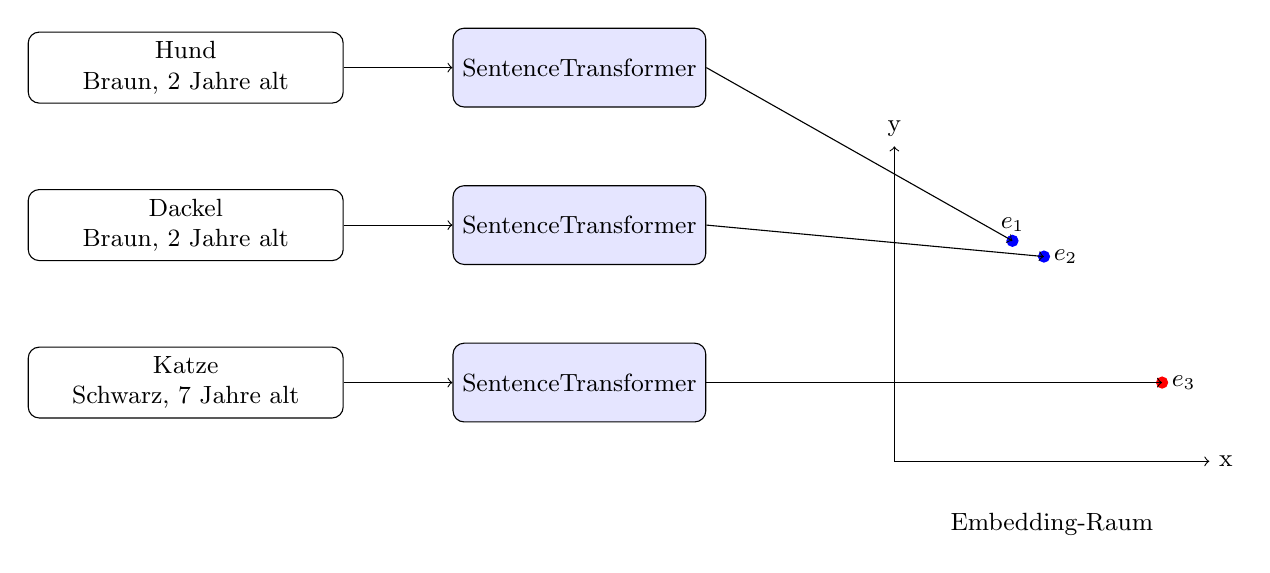
\begin{tikzpicture}[ 
    node distance=1.8cm, every node/.style={font=\small}, 
    textnode/.style=
    { draw, rounded corners, align=center, minimum width=4.0cm, minimum height=0.9cm }, 
    model/.style=
    { draw, fill=blue!10, rounded corners, minimum width=2.5cm, minimum height=1cm } ] 
    % Eingabetexte 
    \node[textnode] (t1) at (0,2) 
    {Hund\\Braun, 2 Jahre alt}; 
    \node[textnode] (t2) at (0,0) 
    {Dackel\\Braun, 2 Jahre alt}; 
    \node[textnode] (t3) at (0,-2) 
    {Katze\\Schwarz, 7 Jahre alt}; 
    % Sentence Transformer 
    \node[model] (m1) at (5,2) 
    {Sentence\\Transformer}; 
    \node[model] (m2) at (5,0) 
    {Sentence\\Transformer}; 
    \node[model] (m3) at (5,-2) 
    {Sentence\\Transformer}; 
    % Pfeile zum Modell 
    \draw[->] (t1) -- (m1); 
    \draw[->] (t2) -- (m2); 
    \draw[->] (t3) -- (m3); 
    % Embedding-Raum 
    \draw[->] (9,-3) -- (13,-3) node[right] {x}; 
    \draw[->] (9,-3) -- (9,1) node[above] {y}; 
    \node at (11,-3.8) {Embedding-Raum}; 
    % Punkte 
    \filldraw[blue] (10.5,-0.2) circle (2pt); 
    \node[above] at (10.5,-0.2) {$e_1$}; 
    \filldraw[blue] (10.9,-0.4) circle (2pt); 
    \node[right] at (10.9,-0.4) {$e_2$}; 
    \filldraw[red] (12.4,-2.0) circle (2pt); 
    \node[right] at (12.4,-2.0) {$e_3$}; 
    % Verbindungslinien 
    \draw[->] (m1.east) -- (10.5,-0.2); 
    \draw[->] (m2.east) -- (10.9,-0.4); 
    \draw[->] (m3.east) -- (12.4,-2.0); 
    \end{tikzpicture} 
    \caption{Prinzipielle Funktionsweise eines Sentence Transformers. Semantisch ähnliche Texte werden auf nahe beieinanderliegende Embeddings abgebildet, während inhaltlich unterschiedliche Texte größere Abstände im Embedding-Raum aufweisen.} 
    \label{fig:sentence_transformer} 
\end{figure}


\subsection{Embedding-Modelle}

\subsection{Triplet Loss}

\subsection{Learning-to-Rank}

Learning-to-Rank (LTR) bezeichnet eine Klasse von maschinellen Lernverfahren, die das Ziel besitzen, die Reihenfolge in einer Ergebnisliste zu optimieren \parencite{liu2009learning}.
Im Gegensatz zu klassischen Klassifikations- oder Regressionsansätzen bewertet Learning-to-Rank keine einzelnen Objekte isoliert, sondern die relative Relevanz dieser Objekte in einer Kandidatenmenge.
Die Aufgabe eines Rankingmodells besteht darin, dass für eine Anfrage die relevanten Dokumente anhand ihrer Merkmale bewertet werden und anschließend in eine Rangliste überführt werden.

\subsection{LambdaRank}

\section{Validierungsansätze}

\subsection{Recall@k} 

Recall@k gehört zu den grundlegenden Bewertungsmetriken des Information Retrievals und beschreibt den Anteil der Anfragen, bei denen mindestens ein relevantes Ergebnis innerhalb der ersten $k$ Rangpositionen gefunden wird \parencite{manning2008ir}. 
Diese Metrik berechnet sich wie folgt: 

\begin{align} 
  Recall@k = \frac{ \# \text{Anfragen mit relevantem Ergebnis in Top-}k }{ \# \text{Anfragen} } 
\end{align} 

mit 

\begin{description} 
    \item[$k$]: Anzahl der betrachteten Rangpositionen 
    \item[$\text{Anfragen mit relevantem Ergebnis in Top-}k$]: Anzahl erfolgreicher Anfragen 
    \item[$\text{Anfragen}$]: Gesamtzahl aller Anfragen 
\end{description} 

Der Wertebereich liegt zwischen 0 und 1. Ein Wert von 1 bedeutet, dass sich für jede Anfrage mindestens ein relevantes Ergebnis innerhalb der Top-$k$ Positionen der Rangliste befindet. 
In Ranking- und Empfehlungssystemen wird Recall@k häufig verwendet, um die praktische Verwendung eines Systems beurteilen zu können.
Der Anwender betrachtet dabei in der Regel nur die ersten Ergebnisse einer Rangliste \parencite{manning2008ir}.

\subsection{Mean Reciprocal Rank} 

Der Mean Reciprocal Rank (MRR) zählt neben Recall@k zu etablierten Bewertungsmetriken des Information Retrievals und wird sowohl in klassischen Suchsystemen als auch in modernen Rankingverfahren eingesetzt \parencite{voorhees1999mrr,zhu2024llmirsurvey}. 
Mit dieser Kennzahl wird die Position des ersten relevanten Ergebnisses innerhalb einer Rangliste bewertet.

Die Berechnung ergibt sich wie folgt:  

\begin{align} 
  MRR= \frac{1}{N} \sum_{i=1}^{N} \frac{1}{rank_i} 
\end{align} 

mit 

\begin{description} 
    \item[$N$] Anzahl der ausgewerteten Anfragen 
    \item[$rank_i$] Rangposition des ersten relevanten Ergebnisses für Anfrage $i$ 
\end{description} 

Der Wertebereich liegt zwischen 0 und 1. Ein hoher Wert zeigt an, dass ein relevantes Ergebnis bereits an einer der vorderen Positionen einer Rangliste erscheint. 
Da frühe Treffer stärker gewichtet werden als spätere Treffer, eignet sich die Kennzahl besonders zur Bewertung der schnellen Auffindbarkeit relevanter Ergebnisse.

\subsection{Normalized Discounted Cumulative Gain} 

Der Discounted Cumulative Gain (DCG) wurde von Järvelin und Kekäläinen zur Bewertung verschiedener Relevanzstufen von Suchergebnissen eingeführt und zählt zu den wichtigsten Bewertungsmetriken für Ranking- und Suchsysteme \parencite{jarvelin2002dcg}. 
Die Kennzahl berücksichtigt sowohl die Relevanz eines Ergebnisses als auch die Position innerhalb der Rangliste. Relevante Ergebnisse auf frühen Rangpositionen leisten dadurch einen höheren Beitrag zur Gesamtbewertung. 

Die Berechnung des DCG erfolgt über 

\begin{align} 
  DCG@k = \sum_{i=1}^{k} \frac{2^{rel_i}-1} {\log_2(i+1)} 
\end{align} 

mit 

\begin{description} 
  \item[$k$] Anzahl der betrachteten Rangpositionen 
  \item[$i$] Rangposition innerhalb der Rangliste 
  \item[$rel_i$] Relevanzwert des Ergebnisses auf Rangposition $i$ 
\end{description} 

Um eine bessere Vergleichbarkeit zu schaffen, findet eine Normierung auf die ideale Rangliste statt. Hieraus ergibt sich der Normalized Discounted Cumulative Gain (nDCG): 

\begin{align} 
nDCG@k= \frac{DCG@k} {IDCG@k} 
\end{align} 
mit 
\begin{description} 
  \item[$DCG@k$] DCG-Wert der betrachteten Rangliste 
  \item[$IDCG@k$] \textit{Ideal Discounted Cumulative Gain}, also der höchstmögliche DCG-Wert, der bei einer idealen Sortierung der Kandidaten nach absteigender Relevanz erreicht würde 
\end{description} 

Der Wertebereich liegt zwischen 0 und 1. Ein Wert von 1 entspricht der optimal möglichen Rangfolge.

\subsection{Hierarchische Bewertungsmetriken} 

Nicht jede fachliche Fehlentscheidung hat in technischen Empfehlungssystemen dieselbe Bedeutung.
Ein Ergebnis kann beispielsweise einer technisch verwandten Produkt- oder Makrofamilie angehören, aber trotz fehlender exakter Übereinstimmung für den Anwender weiterhin von Interesse sein. 
Zur Berücksichtigung solcher Beziehungen werden hierarchische Bewertungsmetriken eingesetzt. 

Diese basieren typischerweise auf dem Discounted Cumulative Gain \parencite{jarvelin2002dcg} und verwenden unterschiedliche Relevanzen in abgestufter Reihenfolge. 

Eine mögliche Relevanzfunktion lautet: 

\begin{align} 
rel = 
\begin{cases} 3,& \text{exakte Übereinstimmung}\\ 2,& \text{gleiche Familie}\\ 0,& \text{keine fachliche Beziehung} 
\end{cases} \end{align} 

Dadurch wird eine Rangliste bevorzugt, welche fachlich ähnliche Kandidaten auf höheren Positionen platziert. 
Hierarchische Bewertungsmetriken eignen sich insbesondere für industrielle Empfehlungssysteme, bei denen zwischen exakter Übereinstimmung und fachlicher Nähe unterschieden werden muss.

\section{Handlungsbedarf}